\subsection{M.PC.VP - Variazione del Piano}
\label{sec:VP}

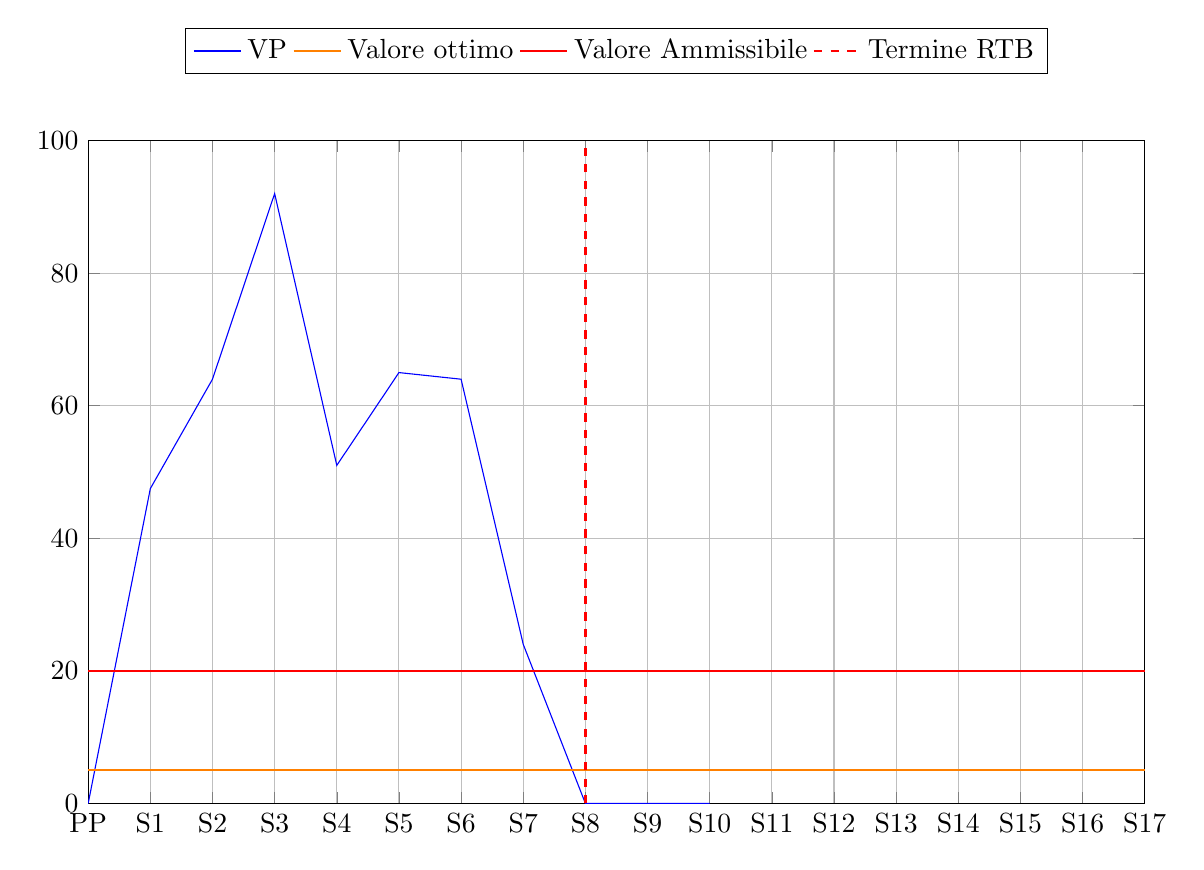
\begin{tikzpicture}
    \begin{axis}[
        width=15cm, height=10cm,
        ymin=0, ymax=100,
        xmin=0, xmax=17,
        xtick={0, 1, 2, 3, 4, 5, 6, 7, 8, 9, 10, 11, 12, 13, 14, 15, 16, 17},
        xticklabels={PP, S1, S2, S3, S4, S5, S6, S7, S8, S9, S10, S11, S12, S13, S14, S15, S16, S17},
        xlabel={},
        ylabel={},
        grid=major,
        scaled ticks=false,
        legend style={at={(0.5,1.1)}, anchor=south, legend columns=-1},
    ]
    \addplot[color=blue] coordinates {(0, 0) (1, 47.5) (2, 64) (3, 92) (4, 51) (5, 65) (6, 64) (7, 24) (8, 0) (9, 0) (10, 0)};
    \addlegendentry{VP}
    \addplot[orange, thick] coordinates {(0, 5) (17, 5)};
    \addlegendentry{Valore ottimo}
    \addplot[red, thick] coordinates {(0, 20) (17, 20)};
    \addlegendentry{Valore Ammissibile}
    \addplot[red, thick, dashed] coordinates {(8, 0) (8, 100)};
    \addlegendentry{Termine RTB}
    \end{axis}
\end{tikzpicture}
\subsubsection{RTB}
Come si vede dal grafico la pianificazione è stata notevolmente errata, è stato pianificato un numero di attività 
eccessivo per ogni \glossario{sprint} portando a un numero elevato di attività non completate, per mancanza di tempo e di impegno da parte del gruppo.
Questo ha portato alla necessità di spostare in avanti la data per \glossario{RTB} inizialmente prevista per completare, durante gli ultimi \glossario{sprint}, le attività precedentemente pianificate.

\paragraph{Sprint 9}
Seguendo le considerazioni fatte in seguito al colloquio con il professore, il gruppo ha deciso di implementare \glossario{issue} molto più piccole e di seguire una pianificazione più realistica.
Questo ha portato a un miglioramento della pianificazione e dell'assegnazione delle attività, portando il valore di \glossario{VP} a 0.

\paragraph{Sprint 10}
Data l'ottima pianificazione e il lavoro svolto dal gruppo  il valore di \glossario{VP} è risultato 0.